\chapter{Bewegliche Objekte}
\section{Abbildungen}
Abbildungen im Text werden
mit Hilfe von \lstinline$includegraphics$ in das Dokument eingef�gt. Das hat den Vorteil, dass man
den Suffix, also den Dateityp, bei der Angabe des Namens weglassen kann. In den meisten
F�llen, bis auf ganz alte Abbildungen, die aus den Quellen f�r  \cite{brill:01} stammen,
gibt es f�r Grafiken eine Version im \datei{png}- oder im \datei{eps}-Format. Damit wird sichergestellt,
dass die Erstellung eines \pdf{}-Dokuments mit Hilfe von \begriff{dvips} oder mit \begriff{pdflatex}
m�glich ist. Stand Juli 2018 wurde auf PDF\LaTeX{} umgestellt, so dass es f�r neue Abbildung ausreicht
das \datei{png}-Format anzubieten.

Auf Abbildungen gibt es immer einen Bezug im Text, sie werden zentriert und die Beschriftung
steht unterhalb der Grafik. Die Abbildung \ref{goldbach} wurde
so in das Dokument eingef�gt:

\begin{lstlisting}{}
\begin{figure}[ht]
\centering
\includegraphics[width=10cm]{\imagePath/tugboat}
\caption{\label{tugboat}Ein sch�nes
Beispiel f�r eine Abbildung}
\end{figure}
\end{lstlisting}
Zentral gibt es ein Verzeichnis \datei{images}, das nochmals
in verschiedene Unterverzeichnisse untergliedert ist. Neben dem Verzeichnis \datei{Misc},
das Abbildungen enth�lt, die allgemein verwendet werden, gibt es Verzeichnisse wie
\datei{Graphentheorie} oder \datei{Funktionen}.

\tip{
Der Name \datei{Misc} des Verzeichnisses stammt vom englischen Begriff \begriff{miscellaneous}.
Die deutsche �bersetzung daf�r ist "`Sonstiges"'.}

\tip{
Eine m�gliche Fehlerquelle, die noch nicht �berall beseitigt wurde ist die Tatsache, dass Verzeichnis-Namen
in der Vergangenheit nicht eindeutig nach Gro�- und Kleinschreibung vergeben wurden. Das ist
unter \windows{} kein Problem, f�hrt aber bei Verwendung auf \linux{} zu Problemen und muss sukzessive
korrigiert werden!
}

\begin{figure}[ht]
\centering
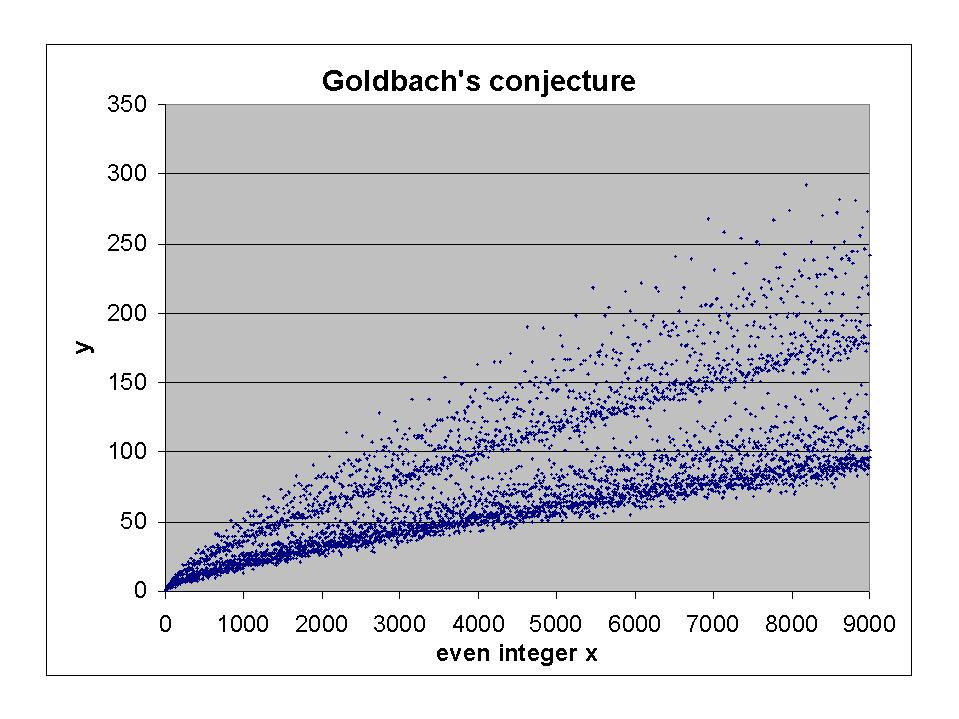
\includegraphics[width=10cm]{\imagePath/goldbach}
\caption{\label{goldbach}Eine Abbildung mit einer Bitmap aus dem Verzeichnis \lstinline$imagePath$}
\end{figure}
Neben Abbildungen, die mit EPS-Grafiken oder Bitmaps\randnotiz{Koordinaten-\\systeme} erstellt werden bietet \LaTeX{} die M�glichkeit mit
Vektorgrafik-Funktionen selbst Abbildungen zu zeichnen. 

Seit September 2018 wird das \LaTeX{}-Paket
\lstinline$xpicture$ eingesetzt. Details findet man in der Dokumentation dieses Pakets
und in \cite{brill_18}. Der Dokumentation zu \datei{mbPDF.sty} sind auch die Abbildungen
\ref{grid} und \ref{polargrid} entnommen.

\begin{figure}[ht]
\definecolor{myblue}{cmyk}{1,1,0,0.5}
\renewcommand{\gridcolor}{myblue}
\renewcommand{\secundarygridcolor}{cyan}
\setlength{\gridthickness}{0.5pt}
\setlength{\secundarygridthickness}{0.1pt}
\renewcommand{\xunitdivisions}{3}
\renewcommand{\yunitdivisions}{3}
\renewcommand{\axeslabelsize}{\footnotesize}
\begin{center}
\setlength{\unitlength}{1cm}
\begin{Picture}(-3.5,-2.5)(3.5,2.5)
\cartesiangrid(-3.4,-2.4)(3.4,2.4)
\end{Picture}
\caption{\label{floats:grid}Ein kartesisches Koordinatensystem mit Gitterlinien (\lstinline$xpicture$)}
\end{center}
\end{figure}

\begin{figure}[ht]
\renewcommand{\runitdivisions}{2}
\setlength{\unitlength}{0.75cm}
\renewcommand{\gridcolor}{magenta}
\begin{center}
\begin{Picture}(-4,-4)(4,4)
\polargrid{3.5}{12}
\end{Picture}
\end{center}
\caption{\label{floats:polargrid}Ein Polarkoordinatensystem mit Koordinatenlinien (\lstinline$xpicture$)}
\end{figure}

Abbildung \ref{floats:grid} wurde mit dem folgenden Quelltext erzeugt:
\begin{lstlisting}{}
\definecolor{myblue}{cmyk}{1,1,0,0.5}
\renewcommand{\gridcolor}{myblue}
\renewcommand{\secundarygridcolor}{cyan}
\setlength{\gridthickness}{0.5pt}
\setlength{\secundarygridthickness}{0.1pt}
\renewcommand{\xunitdivisions}{3}
\renewcommand{\yunitdivisions}{3}
\renewcommand{\axeslabelsize}{\footnotesize}
\begin{center}
\setlength{\unitlength}{1cm}
\begin{Picture}(-3.5,-2.5)(3.5,2.5)
\cartesiangrid(-3.4,-2.4)(3.4,2.4)
\end{Picture}
\end{center}
\end{lstlisting}
Die Abbildung \ref{floats:polargrid} erh�lt man mit den folgenden Zeilen:
\begin{lstlisting}{}
\renewcommand{\runitdivisions}{2}
\setlength{\unitlength}{0.75cm}
\renewcommand{\gridcolor}{magenta}
\begin{center}
\begin{Picture}(-4,-4)(4,4)
\polargrid{3.5}{12}
\end{Picture}
\end{center}
\end{lstlisting}
Das Package \emph{xpicture} setzt \emph{calculator} und \emph{curves}
voraus. Insbesondere das Package \emph{calculator} bietet die M�glichkeit,
mathematische Konstanten und spezielle Funktionen abzurufen und mit Hilfe
von Variablen eigene Berechnungen und Funktionen zu definieren. 
Die Abbildungen \ref{parameter7:zykloide} bis \ref{parameter7:trocho4}
sind mit dem folgenden Source-Code erzeugt worden:

\begin{lstlisting}{}
\begin{figure}[ht]
\COPY{2.0}{\radius}
\SUBTRACTfunction\IDENTITYfunction\SINfunction{\bracketOne}
\SCALEfunction{\radius}\bracketOne{\xfunction}
\SUBTRACTfunction\ONEfunction\COSfunction{\bracketTwo}
\SCALEfunction\radius\bracketTwo{\yfunction}
\PARAMETRICfunction{\xfunction}{\yfunction}{\myparfunction}
\centering
\setlength{\unitlength}{0.175cm}
\begin{Picture}(-36,-0.5)(31,6.5)
\pictcolor{orange}
\linethickness{1pt}
\PlotParametricFunction[48]{\myparfunction}{-16}{15}
\pictcolor{black}
\linethickness{0.5pt}
\xtrivVECTOR(-36.0, 0.0)(31.0, 0.0)
\end{Picture}
\caption{\label{parameter7:zykloide}Eine Zykloide mit $r=2$}

\vspace*{0.2cm}
\COPY{1.5}{\distance}
\SCALEfunction\radius\IDENTITYfunction{\Xone}
\SCALEfunction\distance\SINfunction{\Xtwo}
\SUBTRACTfunction\Xone\Xtwo{\xfunction}
\CONSTANTfunction{\radius}{\Yone}
\SCALEfunction\distance\COSfunction{\Ytwo}
\SUBTRACTfunction\Yone\Ytwo{\yfunction}
\PARAMETRICfunction{\xfunction}{\yfunction}{\myparfunction}
\begin{Picture}(-36,-0.5)(31,6.5)
\pictcolor{orange}
\linethickness{1pt}
\PlotParametricFunction[36]{\myparfunction}{-16}{15}
\pictcolor{black}
\linethickness{0.5pt}
\xtrivVECTOR(-36.0, 0.0)(31.0, 0.0)
\end{Picture}
\caption{\label{parameter7:trocho1}Eine Trochoide mit $r=2$ und $d=1{,}5$}

\vspace*{0.2cm}
\COPY{0.5}{\distance}
\begin{Picture}(-36,-0.5)(31,6.5)
\pictcolor{orange}
\linethickness{1pt}
\PlotParametricFunction[48]{\myparfunction}{-16}{15}
\pictcolor{black}
\linethickness{0.5pt}
\xtrivVECTOR(-36.0, 0.0)(31.0, 0.0)
\end{Picture}
\caption{\label{parameter7:trocho2}Eine Trochoide mit $r=2$ und $d=0{,}5$}

\vspace*{0.2cm}
\COPY{2.5}{\distance}
\begin{Picture}(-36,-1.5)(31,6.5)
\pictcolor{orange}
\linethickness{1pt}
\PlotParametricFunction[48]{\myparfunction}{-16}{15}
\pictcolor{black}
\linethickness{0.5pt}
\xtrivVECTOR(-36.0, 0.0)(31.0, 0.0)
\end{Picture}
\caption{\label{parameter7:trocho3}Eine Trochoide mit $r=2$ und $d=2{,}5$}

\vspace*{0.2cm}
\COPY{3.5}{\distance}
\begin{Picture}(-36,-1.5)(31,6.5)
\pictcolor{orange}
\linethickness{1pt}
\PlotParametricFunction[48]{\myparfunction}{-16}{15}
\pictcolor{black}
\linethickness{0.5pt}
\xtrivVECTOR(-36.0, 0.0)(31.0, 0.0)
\end{Picture}
\caption{\label{parameter7:trocho4}Eine Trochoide mit $r=2$ und $d=3{,}5$}
\end{figure}
\end{lstlisting}

\begin{figure}[ht]
\COPY{2.0}{\radius}
\SUBTRACTfunction\IDENTITYfunction\SINfunction{\bracketOne}
\SCALEfunction{\radius}\bracketOne{\xfunction}
\SUBTRACTfunction\ONEfunction\COSfunction{\bracketTwo}
\SCALEfunction\radius\bracketTwo{\yfunction}
\PARAMETRICfunction{\xfunction}{\yfunction}{\myparfunction}
\centering
\setlength{\unitlength}{0.175cm}
\begin{Picture}(-36,-0.5)(31,6.5)
\pictcolor{orange}
\linethickness{1pt}
\PlotParametricFunction[48]{\myparfunction}{-16}{15}
\pictcolor{black}
\linethickness{0.5pt}
\xtrivVECTOR(-36.0, 0.0)(31.0, 0.0)
\end{Picture}
\caption{\label{parameter7:zykloide}Eine Zykloide mit $r=2$}

\vspace*{0.2cm}
\COPY{1.5}{\distance}
\SCALEfunction\radius\IDENTITYfunction{\Xone}
\SCALEfunction\distance\SINfunction{\Xtwo}
\SUBTRACTfunction\Xone\Xtwo{\xfunction}
\CONSTANTfunction{\radius}{\Yone}
\SCALEfunction\distance\COSfunction{\Ytwo}
\SUBTRACTfunction\Yone\Ytwo{\yfunction}
\PARAMETRICfunction{\xfunction}{\yfunction}{\myparfunction}
\begin{Picture}(-36,-0.5)(31,6.5)
\pictcolor{orange}
\linethickness{1pt}
\PlotParametricFunction[36]{\myparfunction}{-16}{15}
\pictcolor{black}
\linethickness{0.5pt}
\xtrivVECTOR(-36.0, 0.0)(31.0, 0.0)
\end{Picture}
\caption{\label{parameter7:trocho1}Eine Trochoide mit $r=2$ und $d=1{,}5$}

\vspace*{0.2cm}
\COPY{0.5}{\distance}
\begin{Picture}(-36,-0.5)(31,6.5)
\pictcolor{orange}
\linethickness{1pt}
\PlotParametricFunction[48]{\myparfunction}{-16}{15}
\pictcolor{black}
\linethickness{0.5pt}
\xtrivVECTOR(-36.0, 0.0)(31.0, 0.0)
\end{Picture}
\caption{\label{parameter7:trocho2}Eine Trochoide mit $r=2$ und $d=0{,}5$}

\vspace*{0.2cm}
\COPY{2.5}{\distance}
\begin{Picture}(-36,-1.5)(31,6.5)
\pictcolor{orange}
\linethickness{1pt}
\PlotParametricFunction[48]{\myparfunction}{-16}{15}
\pictcolor{black}
\linethickness{0.5pt}
\xtrivVECTOR(-36.0, 0.0)(31.0, 0.0)
\end{Picture}
\caption{\label{parameter7:trocho3}Eine Trochoide mit $r=2$ und $d=2{,}5$}

\vspace*{0.2cm}
\COPY{3.5}{\distance}
\begin{Picture}(-36,-1.5)(31,6.5)
\pictcolor{orange}
\linethickness{1pt}
\PlotParametricFunction[48]{\myparfunction}{-16}{15}
\pictcolor{black}
\linethickness{0.5pt}
\xtrivVECTOR(-36.0, 0.0)(31.0, 0.0)
\end{Picture}
\caption{\label{parameter7:trocho4}Eine Trochoide mit $r=2$ und $d=3{,}5$}
\end{figure}
%
\section{Tabellen}
\begriff{Tabellen} werden mit \datei{table} eingef�gt und haben immer eine Beschriftung, um
im Text darauf Bezug zu nehmen. Die Beschriftung wird als Tabellen-�berschrift
eingef�gt, also oberhalb der Tabelle. Das stammt aus den Projekten mit dem Hanser-Verlag
und wurde seitdem beibehalten. Bei den B�chern wurde die Quelle f�r jede Tabelle
sogar in separate Dateien ausgelagert und in einem Verzeichnis \datei{tables}
zusammengefasst. Dies ist sinnvoll wenn Tabellen sowohl in einem Text als auch
in Folien, die man mit dem \begriff{Beamer}-Paket erstellt, verwendet. So ist sicher gestellt,
dass die Tabelle nur an einer Stelle steht und dass Korrekturen so immer f�r alle Dokumente
wirken, in denen die Tabelle verwendet wird.

\begin{table}[ht]
\centering
\caption{\label{tabelle}Ein Beispiel f�r eine Tabelle}
\begin{tabular}{ll}\hline
\textbf{Erste Spalte}&\textbf{Zweite Spalte}\\\hline
$1$&Eins\\
$2$&Zwei\\\hline
\end{tabular}
\end{table}
Die Tabelle \ref{tabelle}
wurde mit dem folgenden Quelltext eingef�gt:

\begin{lstlisting}{}
\begin{table}[ht]
\centering
\begin{tabular}{ll}\hline
\textbf{Erste Spalte}&\textbf{Zweite Spalte}\\\hline
Erste Spalte&Zweite Spalte\\\hline
$1$&Eins\\
$2$&Zwei\\\hline
\end{tabular}
\end{table}
\end{lstlisting}
Eintr�ge in den Spalten sind meist linksb�ndig. Das muss man nicht beibehalten, aber
die Ausrichtung von Eintr�gen sollte immer konsistent sein.
